\PassOptionsToPackage{unicode=true}{hyperref} % options for packages loaded elsewhere
\PassOptionsToPackage{hyphens}{url}
%
\documentclass[]{article}
\usepackage{lmodern}
\usepackage{amssymb,amsmath}
\usepackage{ifxetex,ifluatex}
\usepackage{fixltx2e} % provides \textsubscript
\ifnum 0\ifxetex 1\fi\ifluatex 1\fi=0 % if pdftex
  \usepackage[T1]{fontenc}
  \usepackage[utf8]{inputenc}
  \usepackage{textcomp} % provides euro and other symbols
\else % if luatex or xelatex
  \usepackage{unicode-math}
  \defaultfontfeatures{Ligatures=TeX,Scale=MatchLowercase}
\fi
% use upquote if available, for straight quotes in verbatim environments
\IfFileExists{upquote.sty}{\usepackage{upquote}}{}
% use microtype if available
\IfFileExists{microtype.sty}{%
\usepackage[]{microtype}
\UseMicrotypeSet[protrusion]{basicmath} % disable protrusion for tt fonts
}{}
\IfFileExists{parskip.sty}{%
\usepackage{parskip}
}{% else
\setlength{\parindent}{0pt}
\setlength{\parskip}{6pt plus 2pt minus 1pt}
}
\usepackage{hyperref}
\hypersetup{
            pdfborder={0 0 0},
            breaklinks=true}
\urlstyle{same}  % don't use monospace font for urls
\usepackage{graphicx,grffile}
\makeatletter
\def\maxwidth{\ifdim\Gin@nat@width>\linewidth\linewidth\else\Gin@nat@width\fi}
\def\maxheight{\ifdim\Gin@nat@height>\textheight\textheight\else\Gin@nat@height\fi}
\makeatother
% Scale images if necessary, so that they will not overflow the page
% margins by default, and it is still possible to overwrite the defaults
% using explicit options in \includegraphics[width, height, ...]{}
\setkeys{Gin}{width=\maxwidth,height=\maxheight,keepaspectratio}
\setlength{\emergencystretch}{3em}  % prevent overfull lines
\providecommand{\tightlist}{%
  \setlength{\itemsep}{0pt}\setlength{\parskip}{0pt}}
\setcounter{secnumdepth}{0}
% Redefines (sub)paragraphs to behave more like sections
\ifx\paragraph\undefined\else
\let\oldparagraph\paragraph
\renewcommand{\paragraph}[1]{\oldparagraph{#1}\mbox{}}
\fi
\ifx\subparagraph\undefined\else
\let\oldsubparagraph\subparagraph
\renewcommand{\subparagraph}[1]{\oldsubparagraph{#1}\mbox{}}
\fi

% set default figure placement to htbp
\makeatletter
\def\fps@figure{htbp}
\makeatother


\date{}

\begin{document}

\hypertarget{header-n0}{%
\subsection{Data Visualization}\label{header-n0}}

In this project, we use the \emph{Gephi} application to implement the
Douban user data visualization. Gephi is an open-source network analysis
and visualization software package written in Java on the NetBeans
platform. It was initially developed by students of the University of
Technology of Compiègne in France.

Considering that the whole dataset is quite slow to run the
visualization program, and the whole dataset will not promise a good
visualization result, we randomly extract a subset of the user dataset
with 246 users, and we will count the following users and followers of
this user, which makes the total number of users is 12678. Besides, we
can build an \emph{adjacent matrix} to represent the directed graph. The
following and followed information can be denoted in a directed graph as
the figure showing. In summary, there're 12678 nodes representing the
users and 16144 edges representing the following information. We will
illustrate some important information the graph can tell.

\hypertarget{header-n6}{%
\subsubsection{Pointed Edge}\label{header-n6}}

The single pointed arrow between \(U_2\) and \(U_1\) suggests that
\(U_2\) follows \(U_1\) but \(U_1\) does not follow \(U_1\). Also, the
double pointed arrow between \(U_1\) and \(U_3\) means that these two
users follow each other.\\

\begin{figure}
\centering
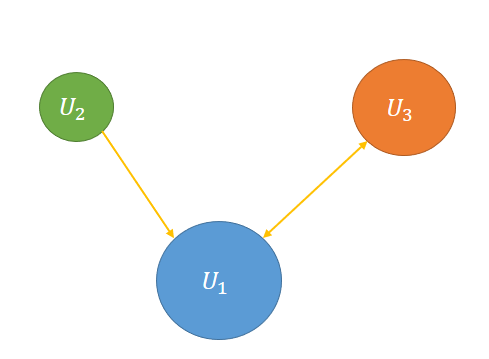
\includegraphics{D:/Doc-1718/Social Network Mining/Fudan-Social_Network_Mining/Doc/report/report/1.png}
\caption{}
\end{figure}

\hypertarget{header-n13}{%
\subsubsection{Node Size}\label{header-n13}}

As you can see from the figure, the sizes of these three nodes are
different. We use the size information to denote the \emph{In-Degree}
rather than just degree. In this situation, users with more fans or
followers can have a big size.

\hypertarget{header-n16}{%
\subsubsection{Node Color}\label{header-n16}}

In this project, a quite meaningful feature of the visualization is the
color. We are not coloring the nodes randomly, in contrast, we use
different colors to represent different communities. That is, we
implement a community division algorithm through the data visualization.
We introduce the Fast Unfolding algorithm to make it. Before we
demonstrate the algorithm, we will first introduce the Community
Division task.

\hypertarget{header-n19}{%
\paragraph{Community Division}\label{header-n19}}

The main goal of the community division is to make the connection in the
samecommunity more dense while make the connection among different
communities more sparse. This can ``split'' the graph into several parts
in general based on their following and followed information.\\

\hypertarget{header-n22}{%
\paragraph{Modularity}\label{header-n22}}

Broadly speaking, modularity is the degree to which a system's
components may be separated and recombined, often with the benefit of
flexibility and variety in use. Modularity is quite an important concept
in social network mining. It describes how meaningful the community
division algorithm is. We can get the modularity as

\[Q =Σ_c  [ \frac{Σ_{in}}{2m}−(\frac{Σ_{tot}}{2m})^2]\]

If a community division is reasonable, it should have a relatively
higher modularity.

\hypertarget{header-n28}{%
\paragraph{Fast Unfolding Algorithm}\label{header-n28}}

\begin{figure}
\centering
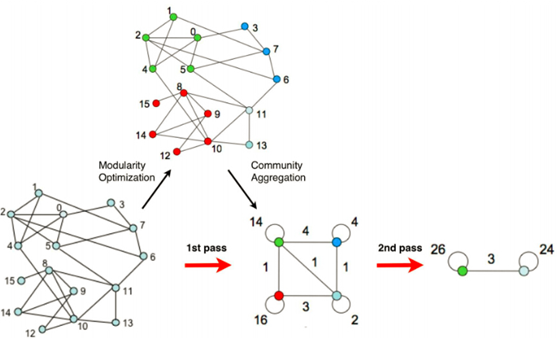
\includegraphics{C:/Users/Leon/OneDrive/DataScience/7_Social Network Mining/Fudan-Social_Network_Mining/Report/2.png}
\caption{}
\end{figure}

We will illustrate the algorithm as following steps.

\begin{enumerate}
\def\labelenumi{\arabic{enumi}.}
\item
  Initialization\\

  Just make all the nodes belonging to different communities. That is,
  if we have N nodes, we have N communities initially.
\item
  Modularity Optimization

  For each node, try to divide each point into the community where its
  neighboring point is located, and calculate the degree of module at
  this point. Judging whether or not the modularity before and after the
  division is increased, if it is yes, then accept this division.
\item
  Community Aggregation

  This is the core of the algorithm. In this step, we will turn all the
  nodes in a same community into one new big node. 
\item
  Iteration

  Iterate the algorithm until the directed graph does not change.
\end{enumerate}

Using such algorithms and all the methods above, we can get the Data
Visualization result as follows:

\begin{figure}
\centering
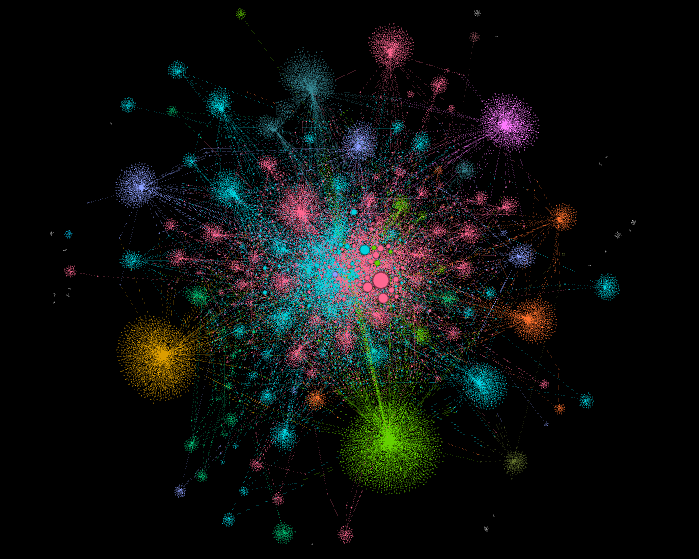
\includegraphics{C:/Users/Leon/OneDrive/DataScience/7_Social Network Mining/Fudan-Social_Network_Mining/Report/3.png}
\caption{}
\end{figure}

And

\begin{figure}
\centering
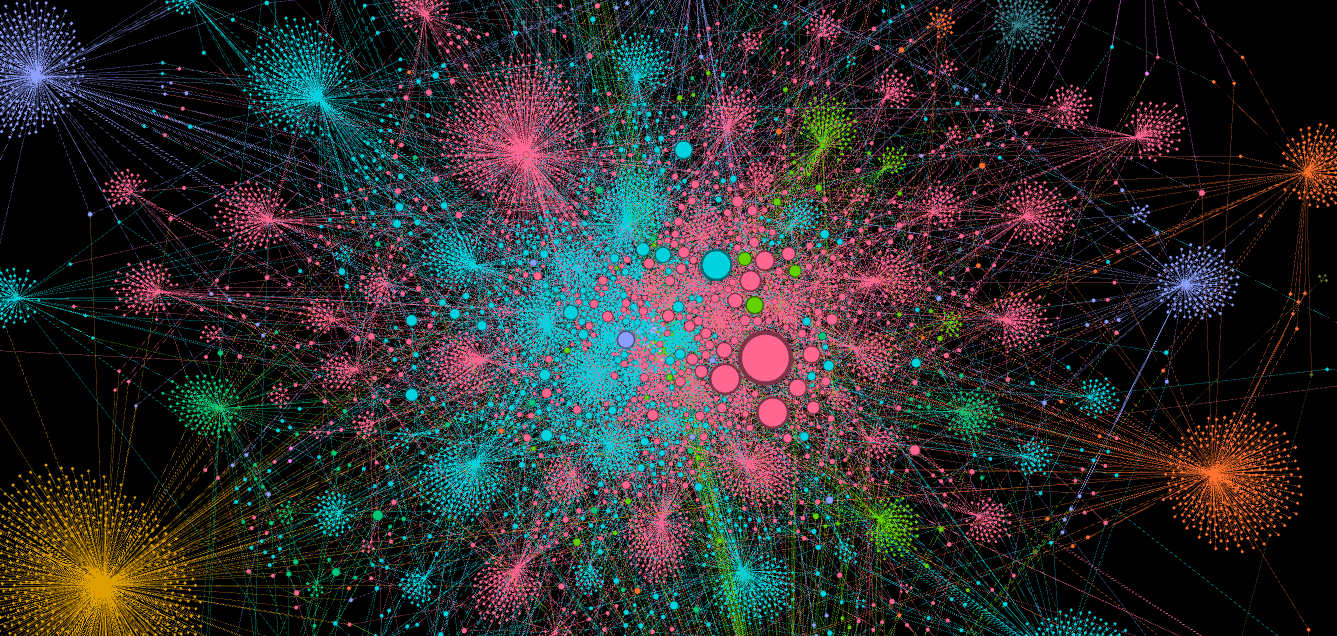
\includegraphics{C:/Users/Leon/OneDrive/DataScience/7_Social Network Mining/Fudan-Social_Network_Mining/Report/5.png}
\caption{}
\end{figure}

Different colors denote different community. And we can know that the
biggest pink node in the middle has the most followers.

\begin{figure}
\centering
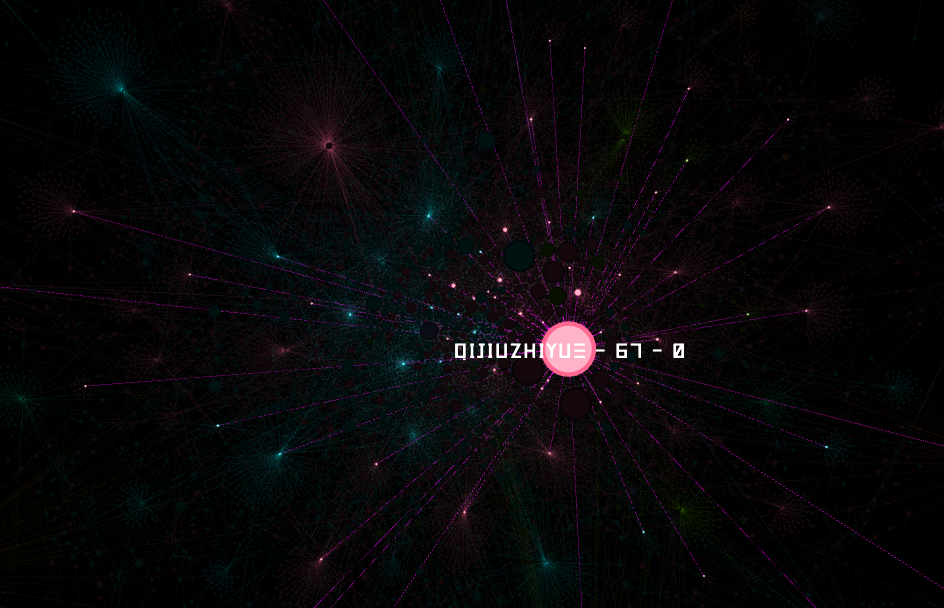
\includegraphics{C:/Users/Leon/OneDrive/DataScience/7_Social Network Mining/Fudan-Social_Network_Mining/Report/6.png}
\caption{}
\end{figure}

Zoom in, we can find the user's information: user's ID, number of
followers and number of following. Besides, we highlight all the related
nodes for ease of observation.

\begin{figure}
\centering
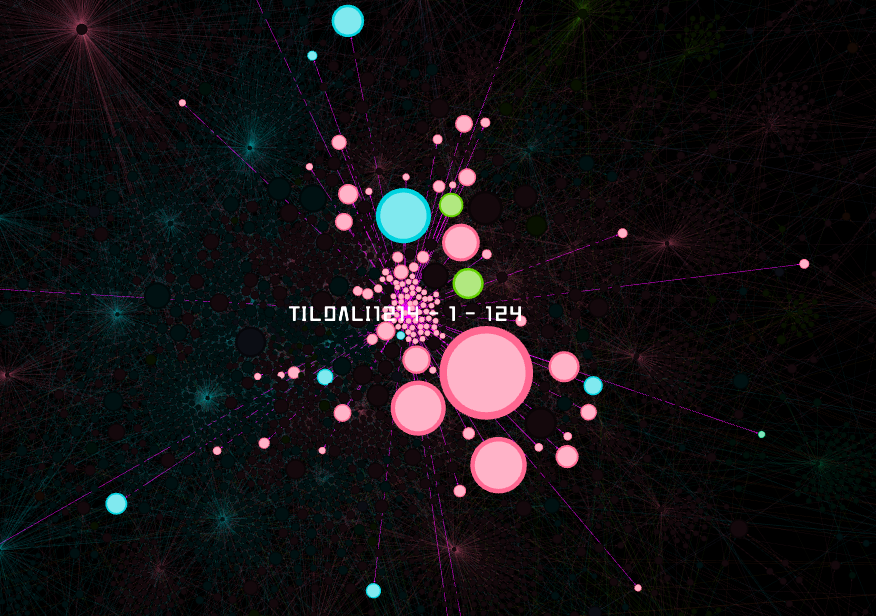
\includegraphics{C:/Users/Leon/OneDrive/DataScience/7_Social Network Mining/Fudan-Social_Network_Mining/Report/4.png}
\caption{}
\end{figure}

\end{document}
